\section{Silicon Pad Sensor Prototypes for the CMS Endcap Calorimeter Upgrade}
\label{sec:sensors}

The CMS high granularity calorimeter will be made of more than \SI{600}{\metre\squared} of planar DC-coupled silicon pad sensors.
The sensors are fabricated as 8'' hexagonal wafers to optimise the use of the circular wafer as which the silicon crystals are grown.
Motivated by empiric evidence of superior noise performance with respect to n-type sensors~\cite{Adam_2017}, p-type doping of their bulk was chosen.
Each HGCAL silicon sensor is segmented into several hundred pads that constitute the sensitive units. 
The majority of those pads are shaped as symmetric hexagons whereas special non-hexagonal structures fill out the wafer periphery.
All pads on a wafer are enclosed and protected from external disturbance by a guard ring.\newline
In this work, full-hexagonal wafer prototype sensors of the so-called low-density (LD) and high-density (HD) designs were irradiated with neutrons and electrically qualified.
Their design is illustrated in~\ref{fig:Sensors}.

\begin{figure}[h]
	\centering
	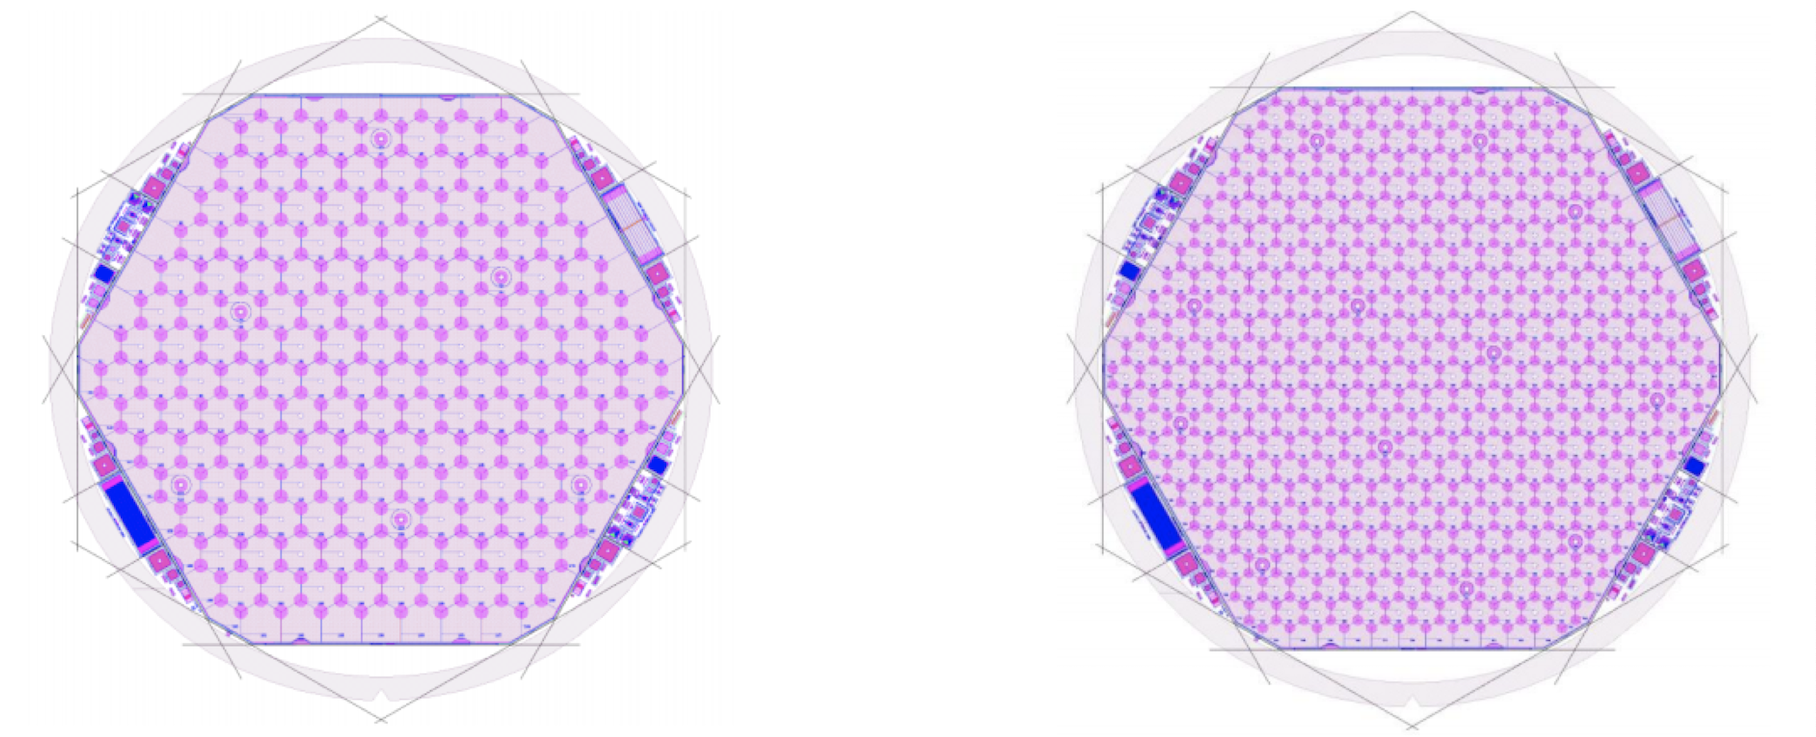
\includegraphics[width=0.75\textwidth]{figures/sensor_layouts.png}
	\caption{
        Layout of the tested 8'' prototype silicon sensors with the low-density (left) and the right-density design (right).
        The test structures at the edges are not relevant for this work and were removed.
	}
	\label{fig:Sensors}
\end{figure}

The LD sensors were produced from physically thinned p-type float zone silicon wafers.
They are segmented into 198 pads, where full hexagonal pads are about \SI{1.2}{\centi\metre\squared} large, and have an active thickness of \SI{200}{\micro\meter} or \SI{300}{\micro\meter}.
It was found empirically~\cite{hgcal-tdr:2018} that the relative signal degradation is worse the thicker the active area of the silicon sensor is.
Therefore, LD sensors will be installed in regions of intermediate radiation fluences inside HGCAL.
By contrast, regions with the highest fluences will be populated with \SI{120}{\micro\meter}-thick HD sensors.
HD sensors are segmented into 444 pads (full hexagon pad size: \SI{0.5}{\centi\metre\squared}) and are produced from epitaxial on a handle wafer.
Although their active thickness amounts to only \SI{120}{\micro\meter}, the physical thickness of HD sensors is \SI{300}{\micro\metre}.\newline
As it is foreseen for the final design, p-stop structures were added to the tested prototype silicon sensors in this work in order to limit the accumulation of electrons between the sensitive pads.
Those structures were either bound to the single pads (individual p-stop) or shared between neighboring ones (common p-stop)~\cite{Brondolin_2020}.
In addition, the tested prototype sensors differed in their flatband voltage (either \SI{-2}{\volt} or \SI{-5}{\volt}).
Other than that, all production parameters, such as doping concentrations and the composition of the oxide layer, were identical for all prototype sensors discussed in this work.
Differences in the bulk properties are not expected to affect the sensor degradation due to irradiation~\cite{MOLL199987} and are thus not subject of this work.
\newline
Prior to irradiation, the studied sensors were electrically qualified demonstrating their proper functionality.
In particular, full depletion was achieved at bias voltages around \SI{40}{\volt} ($\pm\SI{5}{\volt}$) for \SI{120}{\micro\metre} sensors, and around \SI{280}{\volt} ($\pm\SI{10}{\volt}$) for \SI{300}{\micro\meter} sensors, respectively. 
Furthermore, per-pad leakage currents of the non-irradiated sensors did not exceed a few nanoamperes, and the total currents over the full wafer remained well below \SI{100}{\micro\ampere}, over the relevant range of bias voltages up to \SI{-850}{\volt} at room temperature (20-\SI{24}{\celsius}). \newline
In general, exposure of silicon sensors to radiation adds impurities to the silicon lattice which affects both the leakage currents and the depletion voltages. 
While the bulk-dominated leakage current density increases proportionally with the fluence, the expected degradation (i.e. increase for p-type sensors) of the depletion voltage is non-trivial and their quantification beyond the scope of this work.
The interested reader is encouraged to consult Refs.~\cite{moll:SiDamages,LINDSTROM200330} for this purpose.